\documentclass{report}
\usepackage[utf8]{inputenc}
\usepackage{amsmath}
\usepackage{amssymb}
\usepackage{amsthm}
\usepackage{pgfplots}
\usepackage{tikz}
\usepackage{float}
\usepackage[danish]{babel}
\usepackage[margin=1.2in]{geometry}
\usepackage{xcolor}
\usepackage{pdfpages}
\usepackage{csquotes}
\usepackage{hyperref}
\renewcommand{\thesubsection}{\thesection.\alph{subsection}}

\title{Opgave 4, uge 4}
\author{Sebastian Winkelmann}
\date{7. oktober 2019}

\begin{document}
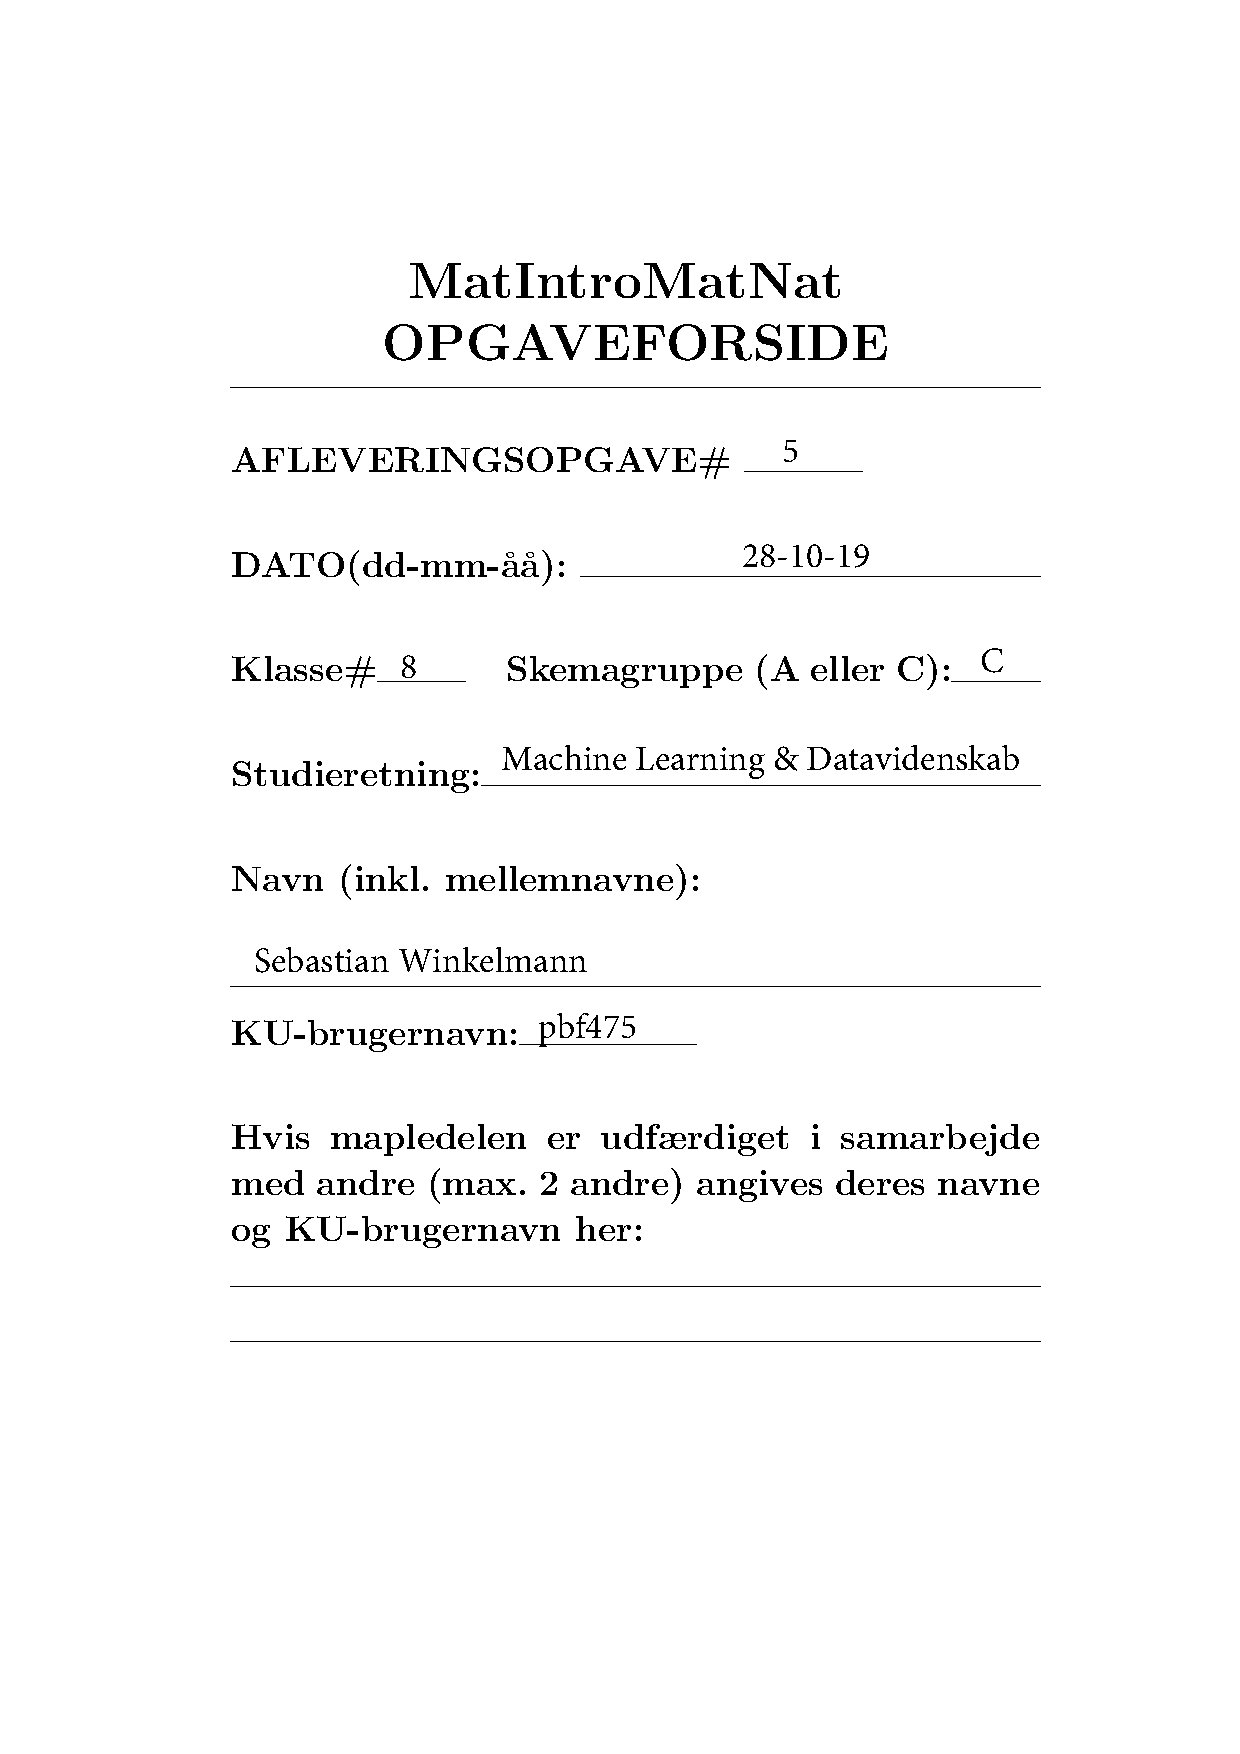
\includepdf{forside.pdf}
\setcounter{chapter}{5}
\section{Største- og mindsteværdi for $f(x,y)$}
\begin{equation}
    f(x,y)=3x+2y^2,\quad A=\{(x,y)\in\mathbb{R}^2|0\leq x\leq2, x-2\leq y\leq x\}
\end{equation}
\subsection{Argumentation}
Vi kan se på udtrykket at funktionen er stigende i intervallet $x>0$. Den mindste $y$-værdi er når $x=0$, da $0-2=-2\leq y\leq 0$, mens den største værdi for $x$ og $y$ er $2$. Således er mængden begrænset, men også lukket/afsluttet da den indeholder alle sine randpunkterne. Af (5.1) fremgår der desuden at $f(x,y)$ er en funktion bestående af $g(x)=3x$ og $h(y)=2y^2$, som begge er kontinuerte funktioner. Trods disse kontinuerte funktionerne $g,h$ ikke har maksima (dog har $h$ et minima), opnår de i domænet både maksimums- og minimumsværdi. Samme egenskab besidder $f(x,y)$. \textbf{Da $A\subset \mathbb{R}^2$ er en lukket, begrænet mængde og $f:A\to\mathbb{R}$ er kontinuert, opnår $f$ -- ifølge ekstremalværdisætningen -- både maksimum og minimum.}
\subsection{Plot}
I maple skriver jeg følgende:
\begin{verbatim}
    f := (x, y) -> 3*x + 2*y^2; s := plot3d(f(x, y), x = 0 .. 2, y = x-2 .. x);
    p := pointplot3d([(0, 0, 0), (2, 2, 14)], symbolsize = 50);
    display([s, p]);
\end{verbatim}
\begin{figure}[H]
    \centering
    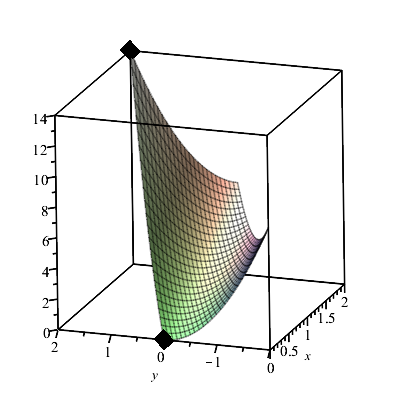
\includegraphics[width=0.5\textwidth]{51b.png}
    \caption{Plot i Maple}
\end{figure}
Maksimumspunktet er ved $f(x,y)=14$, altså i punktet $(2,2,14)$. Minimumspunktet er ved $f(x,y)=0$, som er ved $(0,0,0)$, hvor begge er randpunkter i $A$.

\newpage\section{TKO 2.17 -- Tangentplan}
Når $f$ er $C^1$ og $\mathbf{a}$ et indre punkt i $D_f$, er tangenthyperplanen givet ved den affine funktion\begin{equation}
    h(\mathbf{x})=f(\mathbf{a})+\nabla f(\mathbf{a})\cdot(\mathbf{x}-\mathbf{a})
\end{equation}
\setcounter{subsection}{2}
\subsection{$h(x,y)=(x+y)e^{x-y^2}$ i $\mathbf{c}=(4,-2)$}
$c_x=4,c_y=-2$ er i $D_h=\{(x,y)\in\mathbb{R}^2$ og $x+y$ samt $e^{x-y^2}$ er $C^1$. Jeg finder først gradienten for $h$. Bruger kædereglen for sammensatte funktioner og produktreglen. $\frac{\partial h(x,y)}{\partial x}=(1+0)e^{x-y^2}+(x+y)e^{x-y^2}(1-0)$.
\begin{align*}
    \nabla h(x,y)&=\left(\frac{\partial}{\partial x}h(x,y),\,\, \frac{\partial}{\partial y}h(x,y)\right)=\left((1+x+y)\cdot e^{x-y^2},\,\,e^{x-y^2}+(x+y)\cdot (-2)ye^{x-y^2}\right)\\
    \nabla h(4,-2)&=\left((1+4-2)\cdot e^{4-4},\,\, e^{4-4}+(4-2)\cdot(-2)(-2)e^{4-4}\right)=(3\cdot1, 1+2\cdot4\cdot1)=(3,9)
\end{align*}
Den fundne gradient ved $\mathbf{c}$ kan nu benyttes på (5.2):
\begin{equation}
    h_t(x,y)=\left((4-2)e^{4-4}\right)+(3,9)\cdot(x-4,y+2)=2+3x-12+9y+18=8+3x+9y
\end{equation}
Altså er tangentplanen for $h$ givet ved $h_t(x,y)=3x+9y+8$. Tegnes i Maple ved\begin{verbatim}
    c := pointplot3d([4, -2, h(4, -2)], symbolsize = 15, color = red)
    f := plot3d([h(x, y), 3*x + 9*y + 8], x = 3 .. 5, y = -2.3 .. -1.7, numpoints = 300, 
    color = [h(x, y), grey]); display([c, f])
\end{verbatim}
\begin{figure}[H]
    \centering
    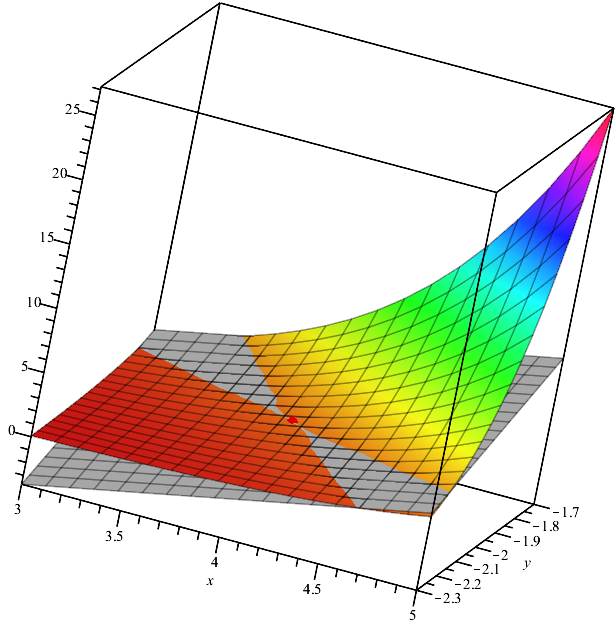
\includegraphics[width=0.6\textwidth]{52c.png}
    \caption{Plot af $h(x,y)$ \texttt{(farvet)}, $h_t(x,y)$ \texttt{(grå)} og $\mathbf{c}=(4,-2)$ \texttt{(rød)}}
\end{figure}
\subsection{$k(x,y)=\frac{x\ln{y}}{\sqrt{1+x^2}}$ i $\mathbf{d}=(0,e)$}
Da $d_x=0,d_y=e$ (hvilket er i $D_k=\{(x,y)\in\mathbb{R}^2|y>0\}$) og både $x\ln{x}$ og $\frac{1}{\sqrt{1+x^2}}$ er $C_1$, kan tangentplanen bruges. Samme fremgangsmåde. Først findes gradienten for $k(x,y)$:
$\frac{\partial k(x,y)}{\partial x}=\frac{1\ln{y}}{\sqrt{1+x^2}}+(-\frac{1}{2})\frac{x\ln{y}}{\sqrt{1+x^2}}2x$
\begin{align*}
    \nabla k(x,y)&=\left(\frac{\ln{y}}{\sqrt{1+x^2}}-\frac{2x}{2}\frac{x\ln{y}}{\sqrt{1+x^2}},\,\,\frac{x}{y\sqrt{1+x^2}}\right)=\left(\frac{\ln{y}}{\sqrt{1+x^2}}-\frac{x^2\ln{y}}{\sqrt{1+x^2}^3},\,\,\frac{x}{y\sqrt{1+x^2}}\right)\\
    \nabla k(0,e)&=\left(\frac{\ln{e}}{\sqrt{1+0^2}}-\frac{0^2\ln{y}}{\sqrt{1+0^2}^3},\,\,\frac{0}{e\sqrt{1+0^2}}\right)=(1,0)
\end{align*}
Den fundne gradient ved $\mathbf{d}$ kan nu benyttes på (5.2):
\begin{equation}
    k_t(x,y)=\frac{0\ln{e}}{\sqrt{1+0^2}}+(1,0)\cdot(x-0,y-e)=0+x-0+0y-0e=x
\end{equation}
Altså er tangentplanen for $k$ givet ved $k_t(x,y)=x$. Tegnes i Maple ved\begin{verbatim}
    d := pointplot3d([0, exp(1), k(0, exp(1))], symbolsize = 15, color = red)
    f := plot3d([k(x, y), x], x = -1 .. 1, y = 0.75*exp(1) .. 1.5*exp(1), numpoints = 300, 
    color = [k(x, y), grey]); display([d, f])
\end{verbatim}
\begin{figure}[H]
    \centering
    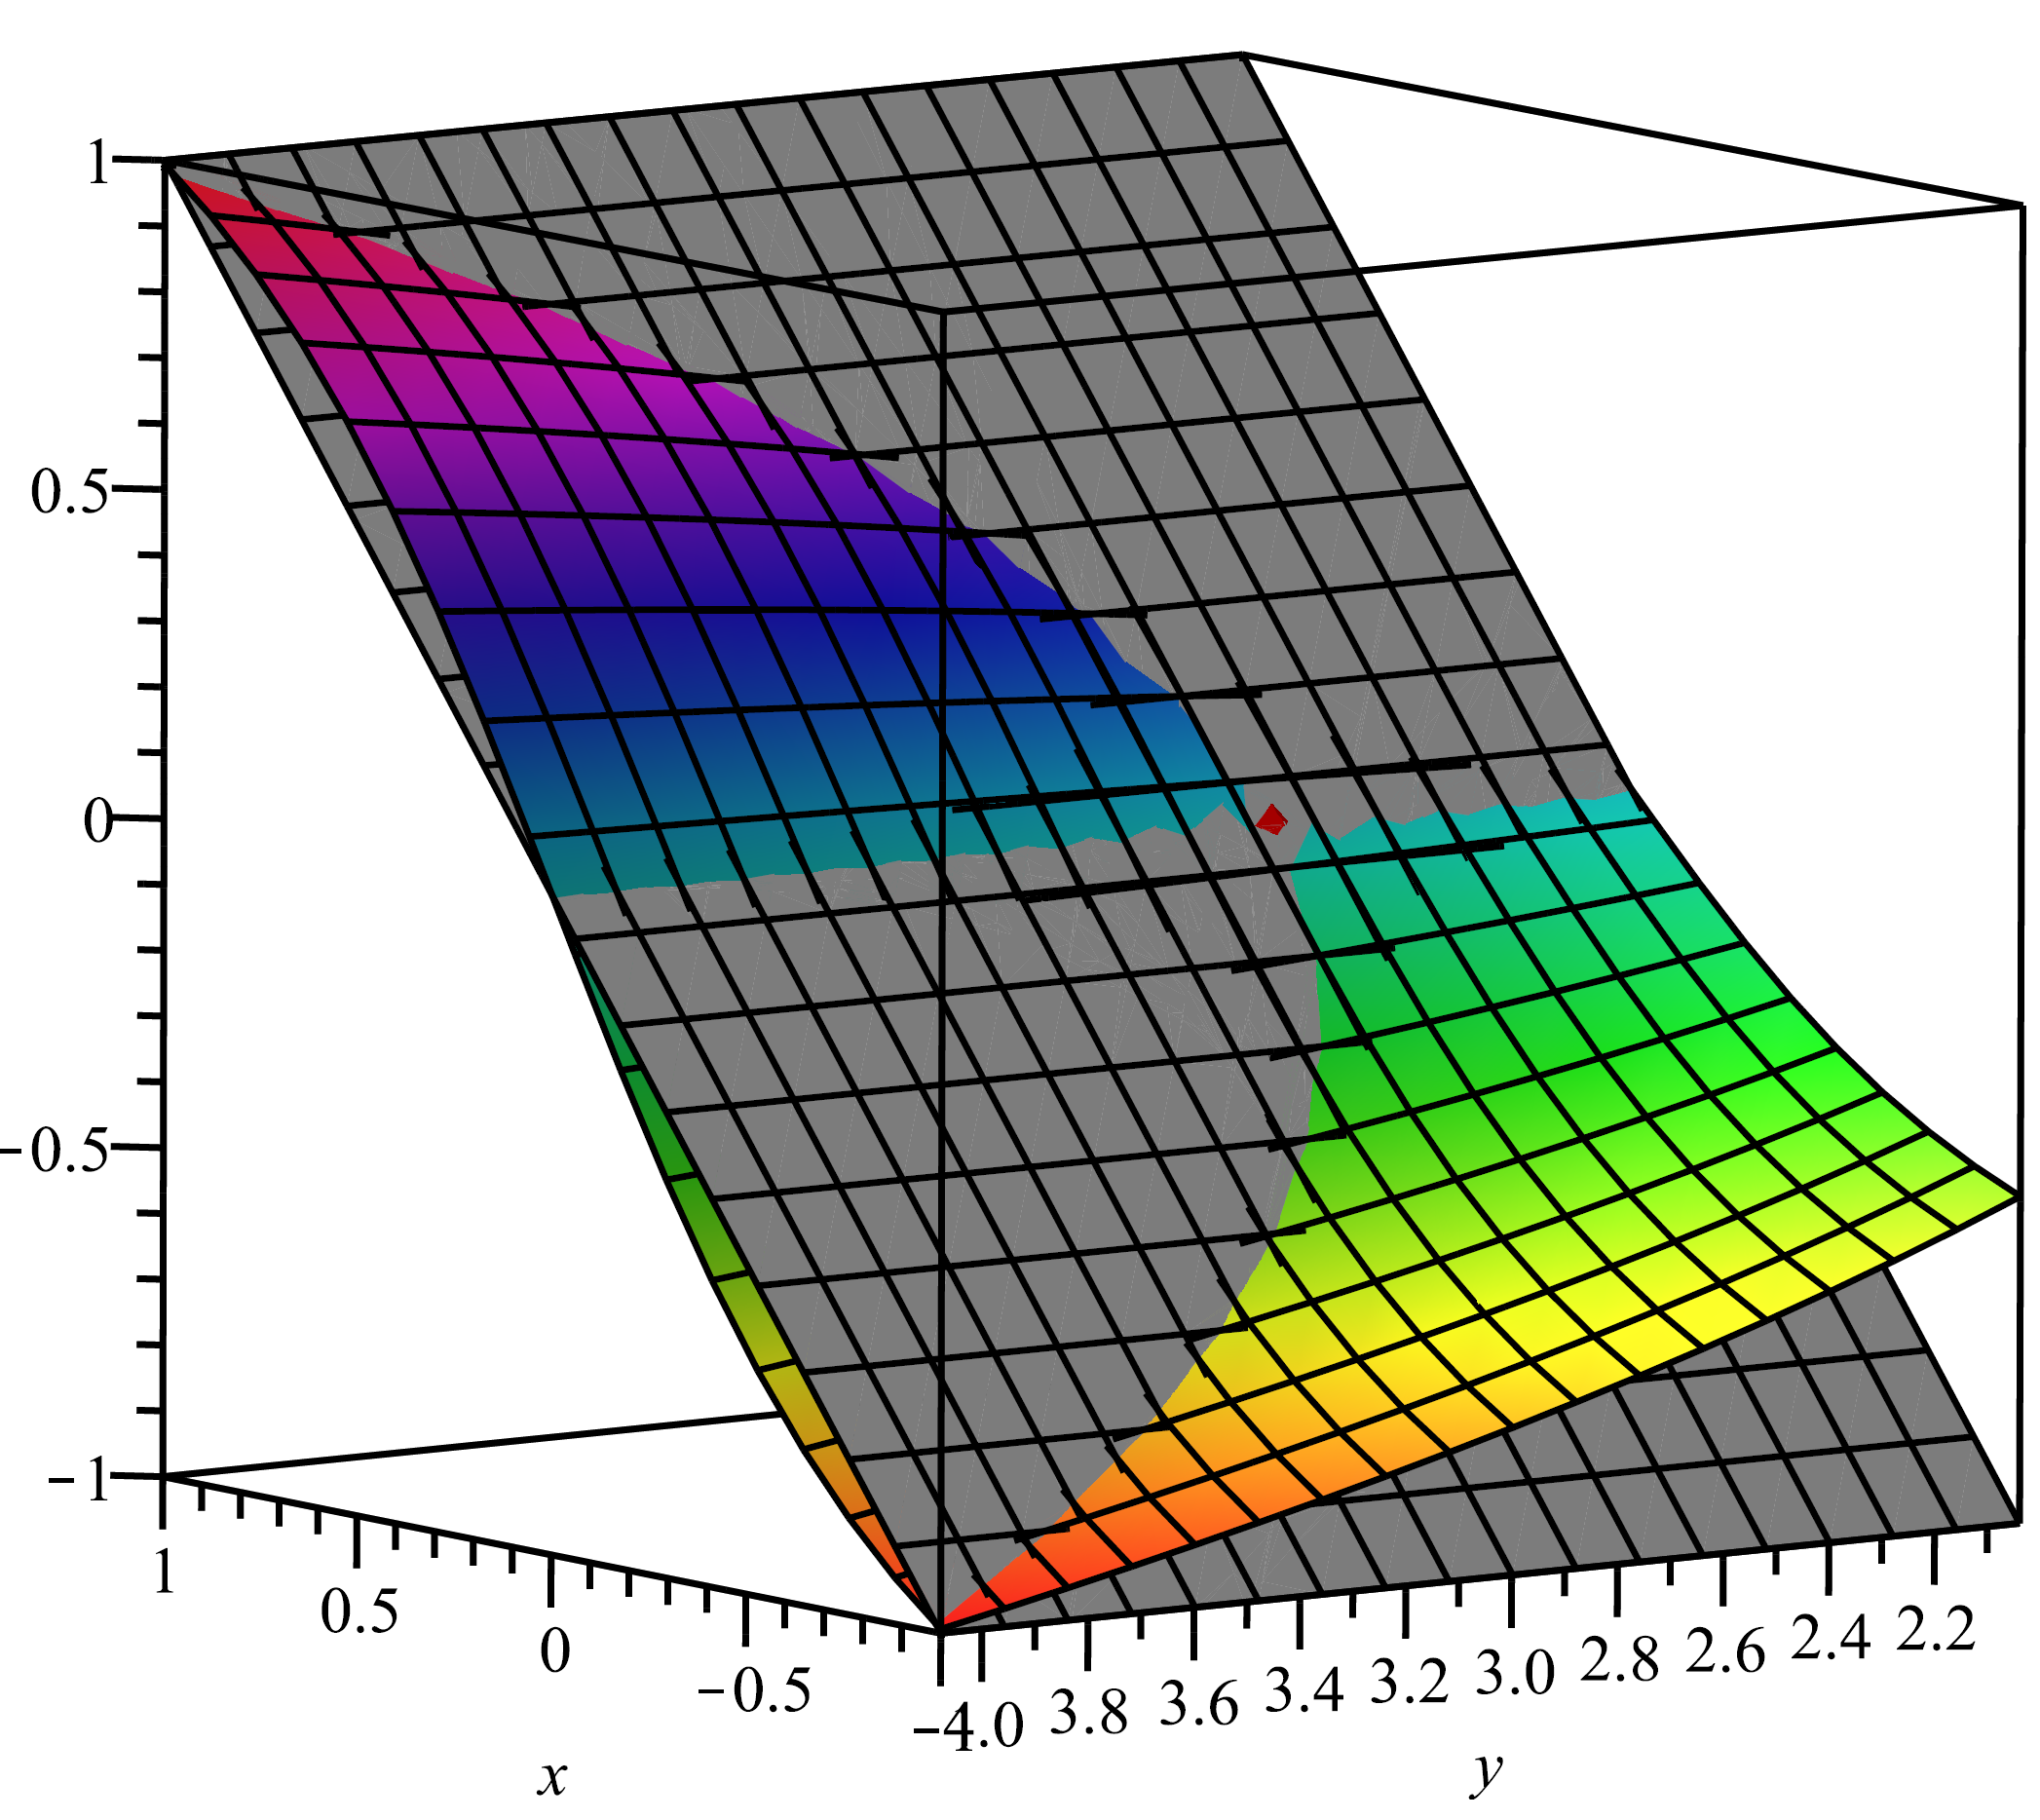
\includegraphics[width=0.6\textwidth]{52d.png}
    \caption{Plot af $k(x,y)$ \texttt{(farvet)}, $k_t(x,y)$ \texttt{(grå)} og $\mathbf{d}=(0,e)$ \texttt{(rød)}}
\end{figure}

\newpage\section{(iii) Homogene funktioner}
$D\subset\mathbb{R}^2$ og $k\in\mathbb{R}$, $f:D\to\mathbb{R}$ er homogen af grad $k$ hvis der for alle $t>0$ og alle $(x,y)\in D$ gælder, at
\begin{equation}
    f(tx,ty)=t^kf(x,y)
\end{equation}
\subsection{Eksempel på homogen funktion af grad $k=3$}
Funktionen $$L(x,y)=x^3+y^3$$er en homogen funktion af grad $k=3$, da $L(tx,ty)=(tx)^3+(ty)^3=t^3L(x,y)$.
\subsection{Vis at $f$ opfylder Eulers ligning}
\begin{equation}
    x\frac{\partial f}{\partial x}(x,y)+y\frac{\partial f}{\partial y}(x,y)=k\cdot f(x,y)
\end{equation}
Kædereglen giver $$\frac{\partial f}{\partial t}(tx,ty)=\frac{\partial f}{\partial x}(tx,ty)\cdot\frac{\partial tx}{\partial t}+\frac{\partial f}{\partial y}(tx,ty)\cdot\frac{\partial ty}{\partial t}=x\frac{\partial f}{\partial x}(tx,ty)+y\frac{\partial f}{\partial y}(tx,ty)$$
Mens $f(tx,ty)=t^kf(x,y)$:
\begin{align*}
    D_1f(tx,ty)t&=t^k\frac{\partial f}{\partial x}(x,y)\implies D_1f=t^{k-1}\frac{\partial f}{\partial x}(x,y)\\
    D_2f(tx,ty)t&=t^k\frac{\partial f}{\partial y}(x,y)\implies t^{k-1}\frac{\partial f}{\partial y}(x,y)\\
    D_3f(tx,ty)&=\frac{\partial}{\partial t}t^kf(x,y)=kt^{k-1}f(x,y)=xD_1f+yD_2f
\end{align*}
Vi kan bruge dette med kædereglen
\begin{align*}
    D_1f(tx,ty)x+D_2f(tx,ty)y&=D_3f(tx,ty)\\
    t^{k-1}\frac{\partial f}{\partial x}x+t^{k-1}\frac{\partial f}{\partial y}y&=kt^{k-1}f(x,y)\\
    \frac{\partial f}{\partial x}x+\frac{\partial f}{\partial y}y&=kf(x,y)
\end{align*}
\subsection{Tjek at funktion fra (a) opfylder Eulers ligning}
Når $L(x,y)=x^3+y^3$ og $k=3$, da gælder der at
\begin{align*}
    x\frac{\partial (x^3+y^3)}{\partial x}+y\frac{\partial (x^3+y^3)}{\partial y}=x\cdot(3x^2)+y(3y^2)=3x^3+3y^3=3\cdot(x^3+y^3)=3\cdot L(x,y)
\end{align*}
Altså opfylder $L(x,y)$ fra (a) Eulers ligning.
\subsection{Fortolkning af $C=\frac{\partial B}{\partial m}$ og $D=-\frac{1}{100}\frac{\partial B}{\partial h}$}
\begin{equation}
    B(m,h)=\frac{m}{h^2}
\end{equation}
$C$ angiver hvordan BMI ændrer sig med hensyn til massen, mens $D$ beskriver ændringen i BMI med hensyn til højden. $C$ er den lineære afhængighed af $m$ for $B$, som viser at jo større $h$, desto langsommere vil BMI'en $B$ stige. $D$ viser en skalering af ændringen af $B$ når $h$ ændres, med ændring af fortegn, så en positiv $D$ medfører negativ hældning, og en negativ $D$ medfører positiv hældning. Da der for ethvert mennesker gælder at $m,h\geq 0$, vil der ved et hvert $m,h$ være en positiv hældning, således at $C,D\geq 0$.
\subsection{Person med vægt $m$, højde $h$ og BMI $B=22$.}
$$m\cdot C+22=100\cdot h\cdot D$$
Det kan omskrives ved at isolere for $22=B$, altså $$m\cdot C+B=100\cdot h\cdot D\implies B=100\cdot-\frac{1}{100}\frac{\partial B}{\partial h}\cdot h-m\cdot\frac{\partial B}{\partial m}=-h\frac{\partial B}{\partial h}-m\frac{\partial B}{\partial m}$$
$\frac{\partial B}{\partial h}=-2\frac{m}{h^3}$ og $\frac{\partial B}{\partial m}=\frac{1}{h^2}$. Dette indsættes
$$B=-h\cdot(-2\frac{m}{h^3})-m\cdot\frac{1}{h^2}=2\frac{m}{h^2}-\frac{m}{h^2}=\frac{m}{h^2}$$
Jeg har hermed vist at $B=\frac{m}{h^2}\Longleftrightarrow m\cdot C+B=100\cdot h\cdot D$. Da dette gælder for alle $B$, må det nødvendigvis også gælde for $B=22$.
\end{document}